\chapter{Algorithm Design}
\label{chapter:algo}
In this chapter the attention will be focused on the design of the most critical aspects of the \emph{Travlendar+} system from the algorithmic point of view. For this reason we decided to support our arguments with some \emph{Flow Diagrams} that clearly explain the main steps of the most complex algorithmic parts.
\\The most critical part of the system is clearly the scheduling algorithm, thus this part is divided in two main phases: the first one aimed at assigning a day to each task with a weekly scope and the second one aimed at assigning a time slot to each task.  

\subsection{Week Scheduler}
\\In the first stage the algorithm will receive as input a set of tasks with any kind of time behaviour but to be scheduled within the same week; on the passed set will be firstly performed a filtering operation which separates the tasks with fixed day behaviour from the others. 
At this point the ones with flexible and variable time behaviour will be assigned a fixed day, trying to uniformly distribute each task with respect to the day load of task and travel time. This will be done using a stochastic approach based on a probability distribution function such as:  

\begin{equation}
    P( t \in d) = \frac{\tau(d) + \beta \sum\limits_{i \in T(d)}{i \rightarrow B(d)} + \gamma t \rightarrow B(d)}
    {\sum\limits_{j \in D}{\tau(j)} + \beta \sum\limits_{j \in D}{\sum\limits_{k \in T(j)}{k \rightarrow B(j)}} + \gamma \sum\limits_{j \in D}{t \rightarrow B(j)}}
\end{equation}  

    \newpage
    where:
    
    \begin{table}[H]
        \centering
        \begin{tabular}{p{2.3cm} p{7cm}}
            \\ $ \Omega$ & is the set of the task in the current week \\
            \\ $ T(d) $  & is the set of task in a given day d \\
            \\ $ D $     & is the set of days for the current week  \\
            \\ $t \in \Omega $ &  \\
            \\ $ d \in D $ & \\
            \\ $ \tau(d)$ & is the sum of the duration time of every task in a given day d  \\
            \\ $ B(d) $ & is the barycenter of the task location for a given day d\\
            \\ $s \rightarrow B(d)$ & is the distance between a task s and the baycenter for a given day d\\
            \\ $\beta, \theta$ & are constants  \\
        \end{tabular}
    \end{table}
    
\\After this stage every task will have a fixed day, thus they will be scanned in order to find evident conflicts between fixed time tasks.
If so, the conflicting tasks will be postponed in the next feasible day at first, if even this solution result unfeasible, then they will be signaled with an error; once the feasibility check ends the algorithm will start to cycle over each day, invoking the subroutine that schedule tasks in a given day (which will be detailed later). 
 The resulting day schedule will be double checked and, if there are no errors, the scheduling proceeds with the next day, until the end of the week is reached. Notice that, if a conflict occurs in the scheduled day, then the algorithm will, at first, try to postpone one of the conflicting tasks to the next feasible day, then it will end signaling the conflicting tasks.   
 
\begin{figure}[H]
    \centering
    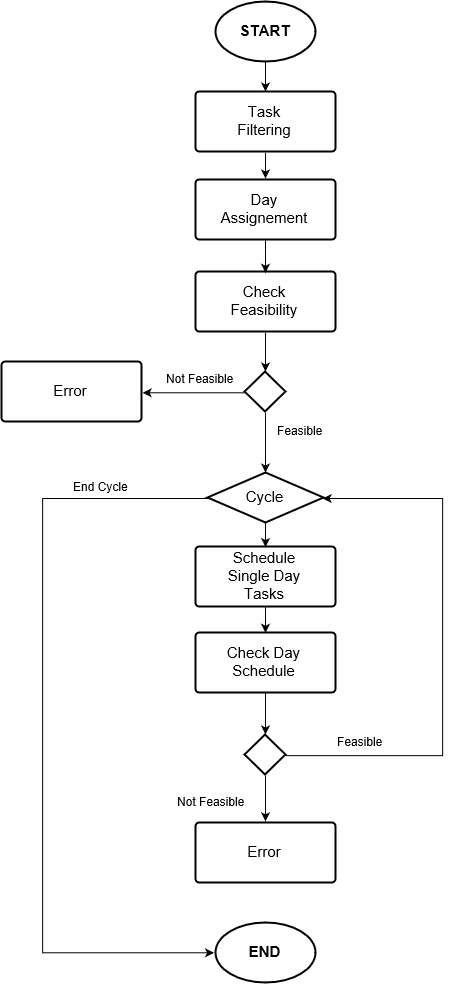
\includegraphics[scale=0.6]{Pictures/FlowDiagram/Algorithm2.png}
    \caption{\emph{Flow Diagram} for the day assignment problem}
    \label{fig:scheduleAlg}
\end{figure}

  

\subsection{Day Scheduler}
\\Now that from an high point of view it's clear how the scheduling algorithm operates, we will better detail how the assignment of time slot to each task in a given day works.
\\The time scheduler algorithm will try to organize the tasks in three main phases: at first the ones with a fixed time slot, then the ones with flexible time slot and finally the ones with a variable time slot.
In each of these phases the scheduling will be based on the Branch and Bound algorithm thus, given a certain task set every possible combination will be explored and evaluated if necessary. For this reason, in the worst case the overall complexity is in the order of $O(\exp(n))$ with n the number of the tasks in the given set. But in average it's proofed, under certain assumptions, that the algorithm has a sub-exponential complexity (see the Reference documents section). 
If during the Branch and Bound the algorithm discovers that a task inevitably conflicts with the others, then depending on the day behaviour of the task different actions will be taken: if day fixed then the algorithm terminates and signals the conflicting task, otherwise it will postpone the task to the next feasible day and continue the day scheduling process, until all the tasks are parsed.


\begin{figure}[H]
    \centering
    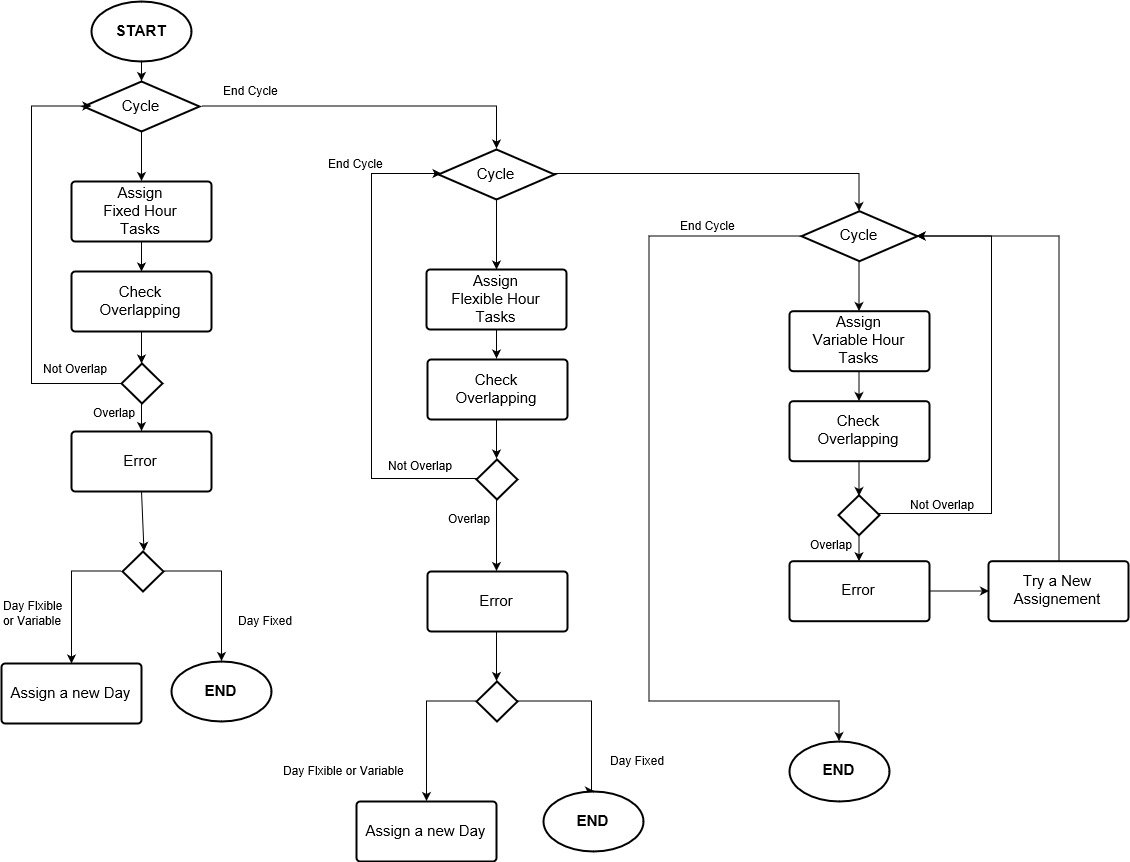
\includegraphics[scale=0.36]{Pictures/FlowDiagram/Algorithm.png}
    \caption{\emph{Flow Diagram} for the schedule algorithm on a single day}
    \label{fig:singleDayAlg}
\end{figure}

